\documentclass[12pt,a4paper]{article}
\usepackage[utf8]{inputenc}
\usepackage{url}
\usepackage{hyperref}
\usepackage{float}
\usepackage[utf8]{inputenc}
\usepackage[english]{babel}
\usepackage{url}
\usepackage{graphicx, capt-of}
\usepackage{titletoc}
\usepackage{setspace}   %Allows double spacing with the \doublespacing command
\usepackage{authblk}
\usepackage{float}
\usepackage{geometry}
\usepackage{textcomp}

\usepackage{caption}
%\geometry{legalpaper, margin=1.2in}
\usepackage[usenames, dvipsnames]{color}
 
%Import the natbib package and sets a bibliography  and citation styles
\usepackage{natbib}
%Import siunitx packages so that tables can be centered
\usepackage{siunitx} 
\usepackage{multirow}
\sisetup{
  round-mode          = places, % Rounds numbers
  round-precision     = 2, % to 2 places
}
\usepackage{rotating}
\usepackage{subcaption}

\newcounter{subfloat}
\renewcommand{\thesubfloat}{\alph{subfloat}}
\newcommand{\image}[2]{%
  \stepcounter{subfloat}%
  \begin{tabular}[t]{@{}c@{}}
  #2 \\
  \end{tabular}%
}

\begin{document}
\pagenumbering{gobble}
{\fontfamily{phv}\selectfont}
\title{\Huge Exploring the Landscape of Glycan Structure\vspace{1cm}\\ \large  MSc Bioinformatics and Theoretical Systems Biology Project\vspace{11cm}}
% * <steven.hargreaves17@ic.ac.uk> 2018-03-20T16:27:53.008Z:
% oh come on now...!
% ^.
\date{}
%\begin{figure}[!b]
%\centering 
%\includegraphics[width=0.5\textwidth]{images/2000px-Imperial_College_London_crest_svg.png}
%\end{figure}
%\begin{figure}[H]
%\centering
%\includegraphics[width=0.5\textwidth]{images/2000px-Imperial_College_London_crest_svg.png}
%\end{figure}
%\vspace{1cm}

\author{\Large Steven Hargreaves\\
\normalsize CID 01453122 \\\vspace{0.5cm}
\normalsize Imperial College London \\
\normalsize Department of Life Sciences}


\maketitle
%\setcitestyle{numbers}
\newpage
\begin{abstract}
\pagenumbering{arabic}
\doublespacing
\noindent RE-WRITE\\
Include some numbers for Sternberg\\
e.g. no. glycans (pre/post filtering steps), no. motifs, assortativity coeffs?
Glycans are tree-like polysaccharides that are frequently found attached to specific sites on eukaryotic cell surface and cellular matrix proteins, with diverse functions including protein folding, cell-cell signaling and immune response. Large databases describing observed glycan structures are now available, which provide an excellent resource for describing and exploring the space of naturally occurring glycans. In this project you will apply tree kernel methods to calculate distances between these structures and thereby develop clustering and data reduction methods to capture the most important differences between subsets of glycans, such as those observed in cancerous vs non-cancerous tissue.
\end{abstract}

\newpage
\begin{center}
\section*{Acknowledgements}
\doublespacing
Many thanks to John Pinney for his supervision and guidance during this project, and Suhail Islam for technical assistance.
\end{center}
\newpage
\tableofcontents
\newpage
\section*{Abbreviations}
\doublespacing
\textit{ABC:} A Big Charlie\\
\textit{DEF:} Dazzling Ear Fountain\\
\addcontentsline{toc}{section}{Abbreviations} %adds it to the table of contents

\newpage
\section*{Glossary}
\addcontentsline{toc}{section}{Glossary}
\label{sec:glossary}
\doublespacing
\noindent{\textit{Clade:} Blah.}\\\\
\textit{Phylogenetic tree:} Blah blah.\\\\
\textit{Archeopteryx.js:} ...phylogenetic trees .\\\\













\newpage
\section{Introduction}
\label{sec:intro}

% ** Max 12 figures and tables\\

% - Set in context of related research here. Don't mention \textit{Drosophila}



% - Describe glycans:\\

% As a minimum, say -- Glycans are chains of sugars, forming tree structures, with links like (blah), which can be alpha/beta etc. They're found (blah), and are used in cell signalling (and blah).\\

\subsection{Glycans}
\label{sec:glycans_description}
Monosaccharides are carbohydrates which cannot be further hydrolyzed to simpler compounds, such as glucose, fructose, and galactose. Glycans, synonymous with polysaccharides, are compounds of monosaccharides (usually more than ten) linked glycosidically \citep{mcnaught1997compendium}, which exist in free form or in covalent complexes with proteins or lipids \citep{doi:10.1093/bioinformatics/btm090}. In both cases, glycans exhibit a tree-like structure, which can be described in terms of its component monosaccharides and the glycosidic links between them. Figure \ref{fig:example_glycan} shows an example glycan, in which the differently coloured and shaped nodes represent different monosaccharides, and the labelled edges represent the glycosidic links.\\

\begin{figure}[H]
\centering 
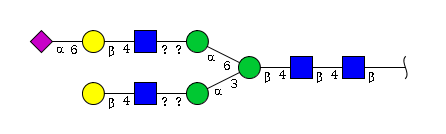
\includegraphics[scale=0.8]{images/glycan_G31576LD.png} 
\caption{An example glycan diagram. The differently coloured and shaped nodes represent different monosaccharides, and the labelled edges represent the glycosidic links between them (image taken from the GlyTouCan repository\protect\footnotemark). Glycosidic links are characterised by the anomericity ($\alpha$ or $\beta$) of carbon 1 on the first monosaccharide, and the carbon number of the non-anomeric carbon on the second monosaccharide. In a number of published glycans, the nature of some glycosidic links has not been satisfactorily established, and is therefore denoted as ambiguous via the use of question mark characters.}
\label{fig:example_glycan}
\end{figure}

\footnotetext{\url{https://glytoucan.org/Structures/Glycans/G31576LD}}

ALSO SHOW MONOSACCHARIDE KEY?\\

When dissolved in an aqueous environment, the monosaccharides (or sugars) of which glycans are comprised, primarily exist in the cyclic (or hemiacetal) form. In this form, the sugars are further characterised by their anomeric \mbox{configurations -- either} the $\alpha$-anomer, with an axial OH-group at carbon 1, or the $\beta$-anomer, with an equatorial OH-group at carbon 1 \citep{SONG2012137}. The glycosidic links between the sugars exist between carbon 1 (the anomeric carbon) of one sugar, and some other, non-anomeric carbon of another. Hence the links are defined by their anomericity ($\alpha$ or $\beta$), and the carbon number of the non-anomeric carbon on the second sugar. This can be seen more clearly in Figure \ref{fig:example_glycan}, where, for example, the XXX (purple diamond) is glycosidically linked via its $\alpha$-anomer carbon 1 to carbon 6 of the XXX (yellow circle), and therefore labelled as `$\alpha$ 6'. This anomericity is significant -- two pairs of monosaccharides glycosidically linked via the same carbons but with different anomeric configurations result in two stereochemically distinct disaccharides, as illustrated in Figure \ref{fig:glycosidic_linkage}. Here, the polymeric form of the maltose disaccharide (starch) is digestible by humans, whereas cellulose, formed from basic repeats of cellobiose, is not \citep{SONG2012137}.\\

% \image{maltose}
% {%
%   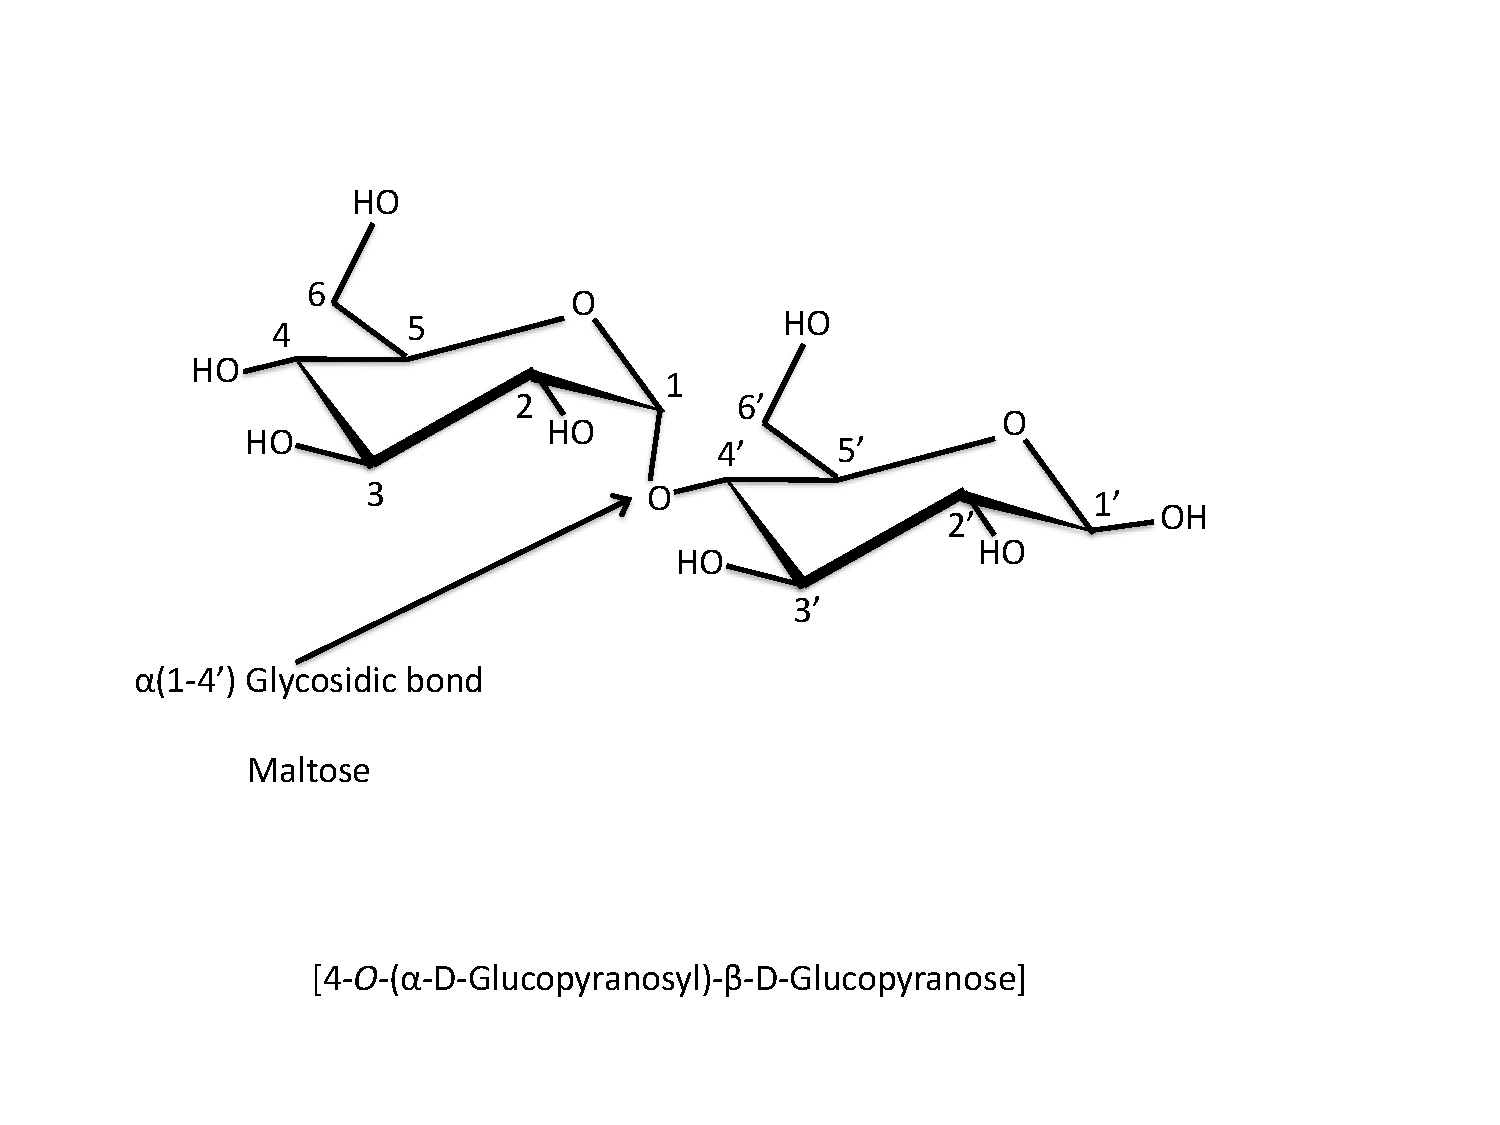
\includegraphics[scale=0.35]{images/glycosidic_linkage_maltose.pdf}%
% }\quad
% \image{cellobiose}{%
%   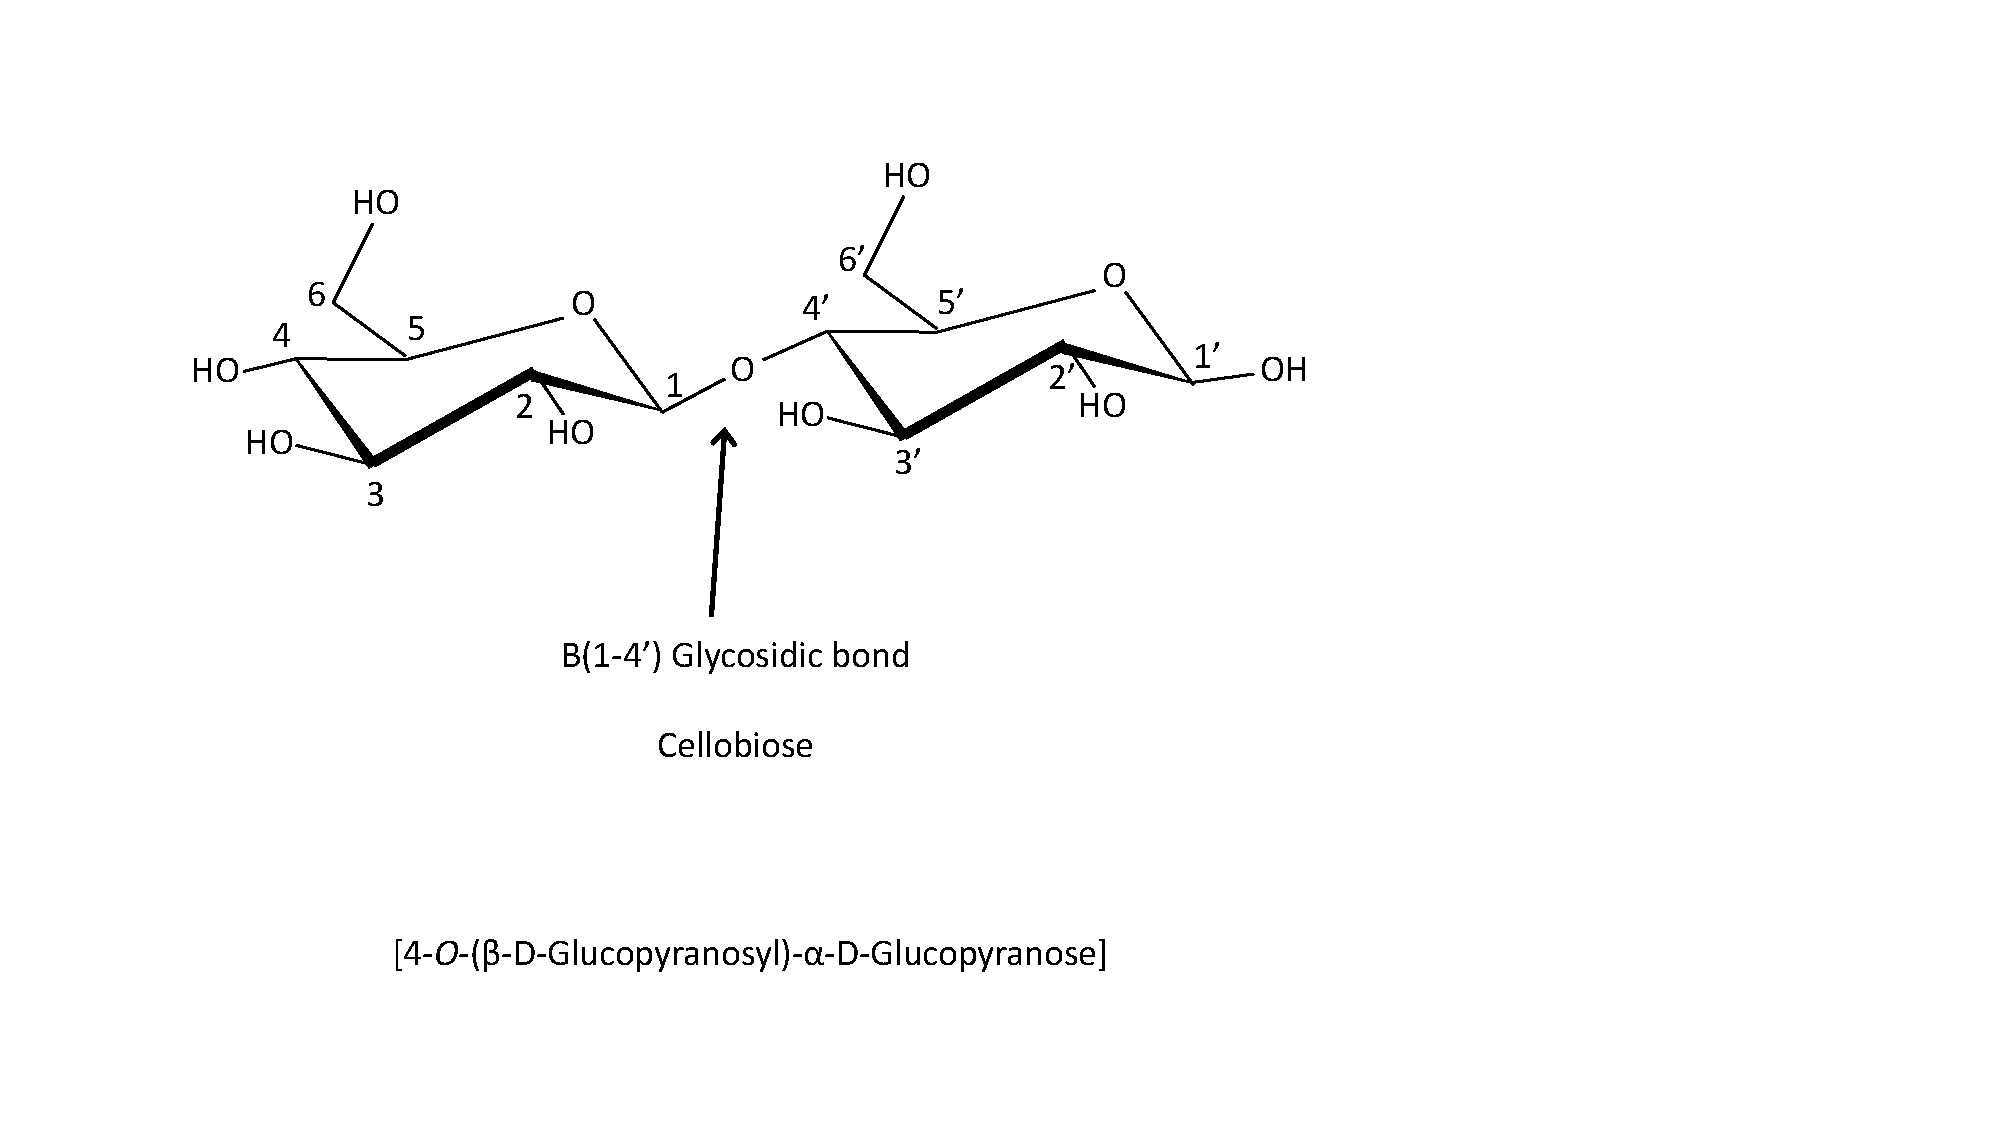
\includegraphics[scale=0.35]{images/glycosidic_linkage_cellobiose.pdf}%
% }\quad
% \captionof{figure}{CROP THESE PDFs, AND BRING THE O and HO closer together in the link.}
% \label{fig:glycosidic_linkage}

\begin{figure*}[ht!]
    \centering
    \begin{subfigure}[t]{1.0\textwidth}
        \centering
        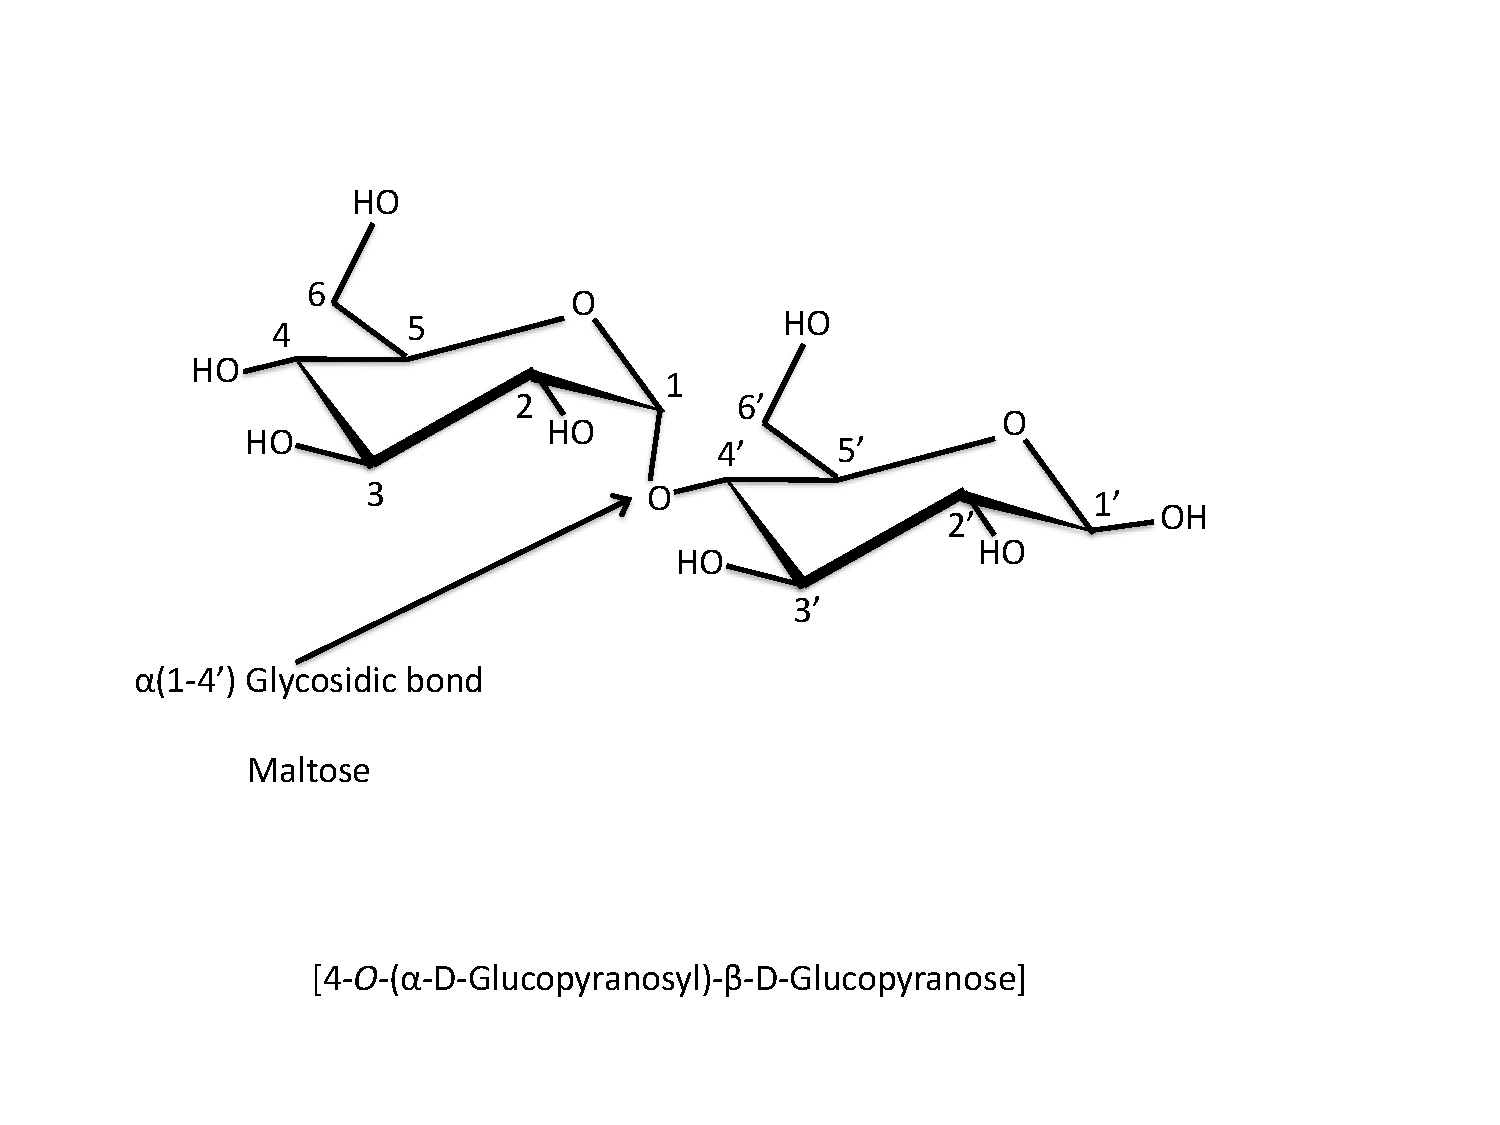
\includegraphics[scale=0.55]{images/glycosidic_linkage_maltose.pdf}
        \caption{Maltose}
    \end{subfigure}%
    \\
    \bigbreak
    ~ 
	\\
    \begin{subfigure}[t]{1.0\textwidth}
        \centering
        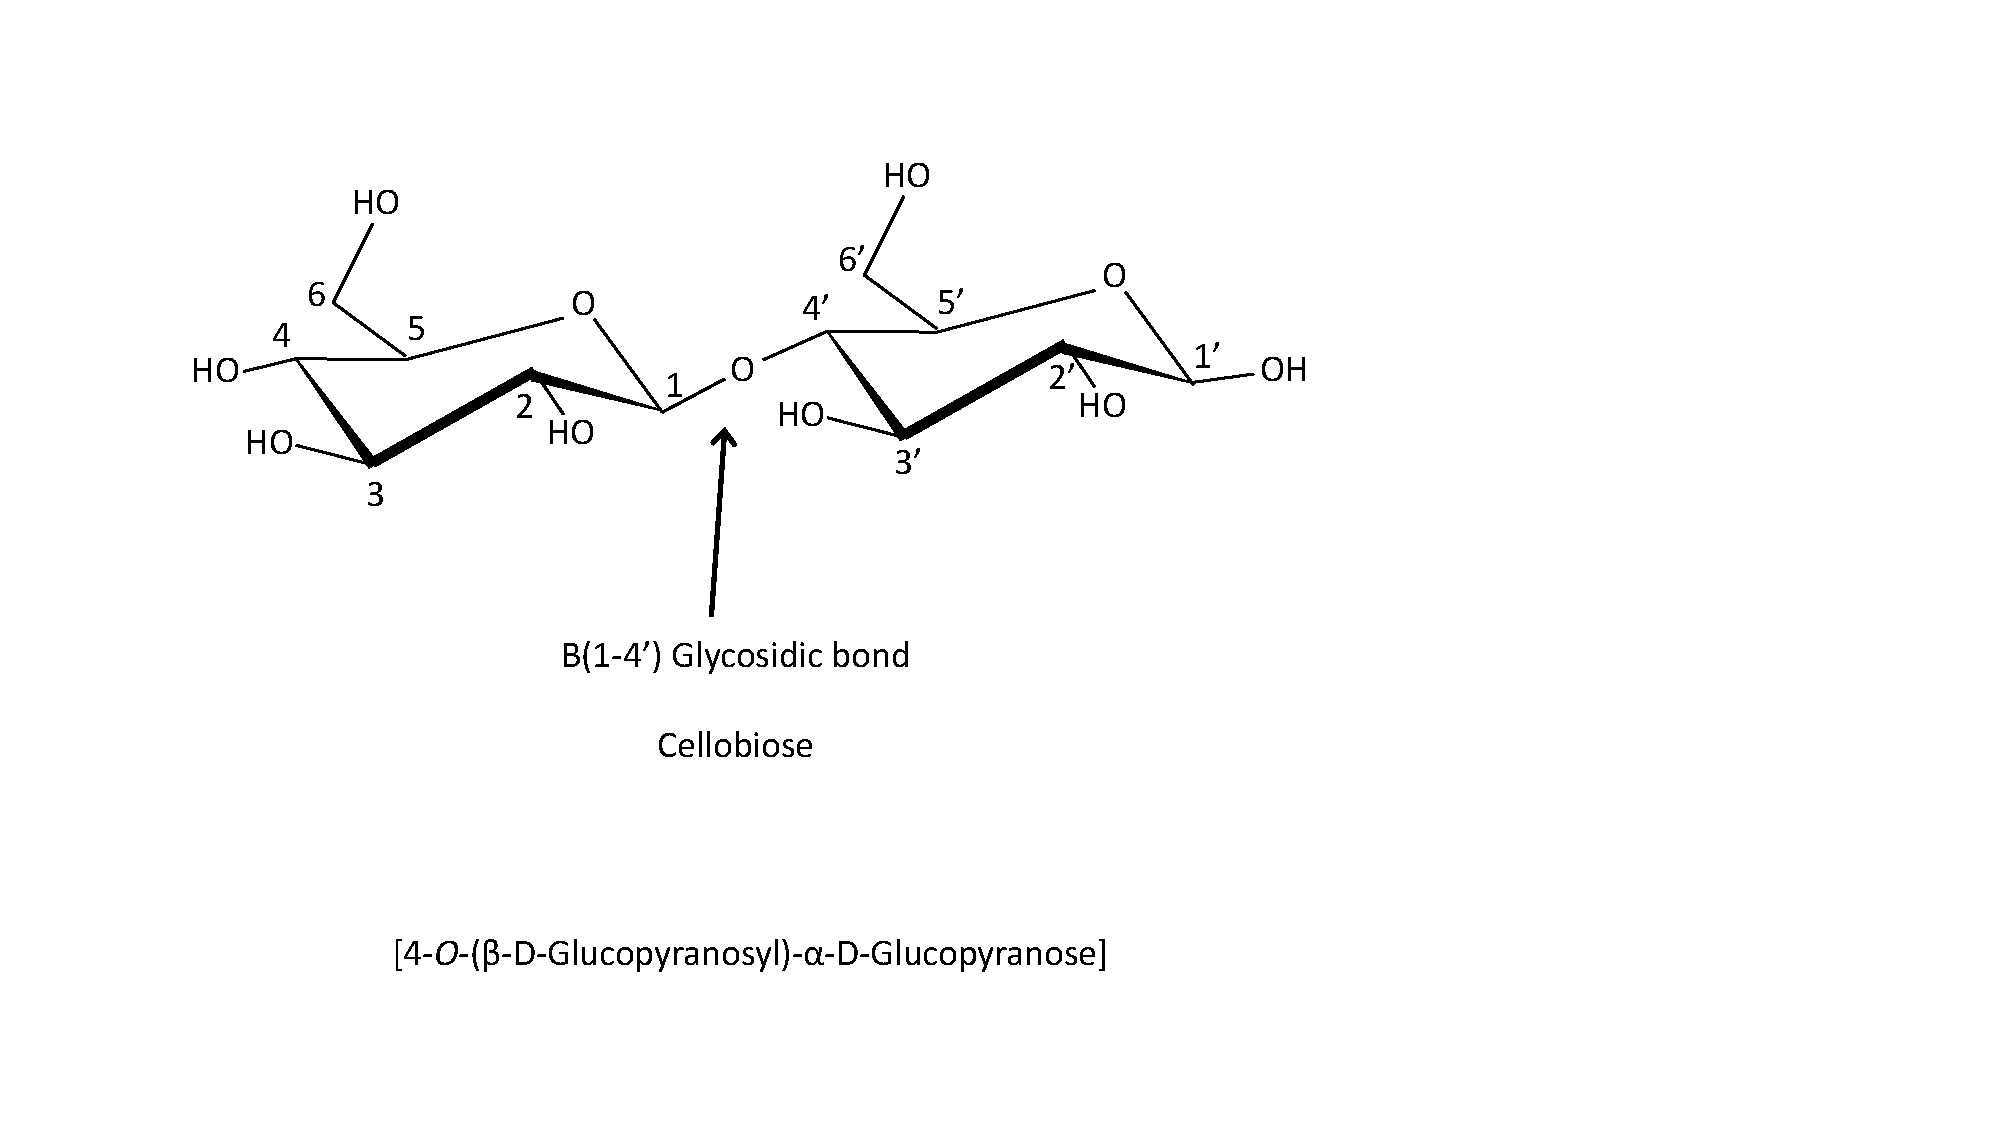
\includegraphics[scale=0.55]{images/glycosidic_linkage_cellobiose.pdf}
        \caption{Cellobiose}
    \end{subfigure}
    \caption{FIX THE BETA SYMBOL Pairs of the same monosaccharide (Glucose) glycosidically linked with different anomericity form different disaccharides (a) maltose and (b) cellobiose.}
\label{fig:glycosidic_linkage}
\end{figure*}

When glycans are linked with proteins or lipids, they are characterised as being either N-linked, in which a monosaccharide is attached to a nitrogen atom of a protein \citep{taylor2011introduction}, or O-linked, in which a glycosidic oxygen links the glycoside to the aglycone or reducing end sugar (LOOK FOR AN ALTERNATIVE, CITABLE EXPLANATION OF THIS, E.G. IN ALBERTS OR THE BIG BIOCHEM BOOK).



% (from wikipedia, no citation - "Glycans can be found attached to proteins as in glycoproteins and proteoglycans. In general, they are found on the exterior surface of cells. O- and N-linked glycans are very common in eukaryotes but may also be found, although less commonly, in prokaryotes.")\\

% (more material on wikipedia if you need it)\\
% (lots of useful info here https://www.sciencedirect.com/science/article/pii/B9780444533494002466 including the chemistry of polysaccharides, which might be useful wrt using glycan reactions.)\\

% (Could also use "Sugars, Mono/poly-saccharide definitions in Alberts chapter 2, 'Biochemistry - The chemistry of Life' David Plummer chapter 3")\\














% -- Where do we find them\\
\subsection{Glycan Diversity, Locations and Motifs}
\label{sec:glycan_locations}
In contrast to the type of bonds found in proteins and nucleic acids, the high number of different glycosidic link configurations possible between monosaccharides leads to high variation and structural diversity between glycans, which confer distinctive characteristics to the cell surface where they are typically found \citep{10.1371/journal.pcbi.1002813}.
There are a total of 105050 distinct glycan structures present in the GlyTouCan\footnote{\url{https://glytoucan.org/}} database. Glycans do however share some common sub-structures, known as motifs. For example, the glycan structure represented in Figure \ref{fig:example_glycan} contains the `N-Glycan core basic' motif, which is displayed in Figure \ref{fig:N-Glycan core basic}. There are just 61 motifs presently listed in the GlyTouCan database - the full list (with diagrams) is available via the footnote link\footnote{\url{https://glytoucan.org/Motifs/listAll}}.

STATE / SHOW THE THREE MAJOR MOTIF TYPES (see wiki / glytoucan)

\begin{figure}[H]
\centering 
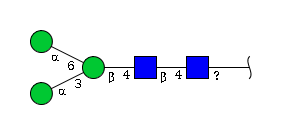
\includegraphics[scale=0.8]{images/n-glycan_core_basic.png} 
\caption{The `N-Glycan core basic' glycan motif, which can also be seen as part of the structure of the glycan shown in Figure \ref{fig:example_glycan}.}
\label{fig:N-Glycan core basic}
\end{figure}









% -- What do they do\\
\subsection{Glycan Function}
\label{sec:glycan_function}
Evidence has been found relating glycans to numerous important biological functions, including immune reaction, protein stabilization, and cell signalling \citep{bucior2004carbohydrate}, tumour progression \citep{fuster2005sweet}, and embryogenesis \citep{rosa2002functional}. Some pathogenic bacteria and viruses have been shown to infect their hosts via glycan-receptor interactions \citep{cossart2004bacterial, sacks2001molecular}, whilst other research has demonstrated that glycan profiles can represent important signatures of disease states \citep{tong2003glycosylation}.

% Recent research has revealed that these glycan profiles can represent important signatures of disease states and thus understanding glycan processing and structures in cells is an important systems biology goal \citep{10.1371/journal.pcbi.1002813}\\

% (glycans) draw attention as the third type of biological chain next to DNA and proteins, since they play key roles in many biological processes such as fertilization (Vo et al., 2003),  immunity (Rudd et al., 2001) and diseases (Birkle et al., 2003; Brockhausen et al., 1998; Hakomori, 2002). It is well known that some pathogenic bacteria and viruses infect their hosts via glycan-receptor interactions (Cossart and Sansonetti, 2004; Sacks and Kamhawi, 2001) \citep{doi:10.1093/bioinformatics/bti666}. \\

% Although a growing body of evidence supports crucial roles for glycans in many cellular processes, including cell-cell communication, immune system, protein interaction or tumor progression (Fuster and Esko, 2005; Varki et al., 1999), \citep{doi:10.1093/bioinformatics/btm090}

% (Glycans) are known to play numerous biological roles related to energy storage and metabolism, protein and lipid modification, cellular structure, signal transduction, as well as mediators of cell-cell interactions and host-pathogen interactions \citep{SONG2012137}




% -- Why are we interested\\

% -- How have they been analysed up until now, and what are the problems in analysing them\\
\subsection{Glycan Analysis}
\label{sec:glycan_analysis}

Given the important and diverse functions attributed to glycans, the ability not just to determine their individual structure, but also to accurately quantify their presence or absence within different cell and tissue types, is of great value. Methods of characterising glycan structures include mass spectral analysis \citep{10.1371/journal.pcbi.1002813}, high performance liquid chromatography, capillary electrophoresis, and nuclear magnetic resonance technology \citep{von2004bioinformatics}, whilst gene expression processing may be used to characterise glycosylation processing enzymes \citep{10.1371/journal.pcbi.1002813}.\\

Glycan analysis though remains highly problematic -- unlike the comparatively mature techniques regularly applied to DNA and RNA analysis, whose nucleotide chains are both linear and contain only 4 elementary components, and which are easy to amplify using (for example) polymerase chain reactions, glycans are tree-like in nature, and the large number of component monosaccharides involved together with the wide range of possible glycosidic links makes glycan structure determination challenging. Consequently only a small number of samples are available for analysis \citep{doi:10.1093/bioinformatics/bti666}.

To mitigate for these experimental shortcomings, in much the same way as sequence homology and multiple alignments may be exploited to construct complete genomes from DNA fragments (REF), there is a need for reliable computational techniques of glycan structure and prevalence prediction. Examples of research towards this end include probabilistic modelling of glycan families \citep{ueda2005probabilistic}, identification of glycan fingerprint differences between prostate cancer cell stages \citep{10.1371/journal.pcbi.1002813}, prediction of glycan structures from gene expression profiles \citep{doi:10.1093/bioinformatics/bti666}, and glycan comparison \citep{aoki2004score, aoki2004kcam} MAYBE A BIT MORE DETAIL ABOUT THESE TECHNIQUES AND RESULTS.




% To understand glycan functions, determination of their structures (sequences) like DNA and proteins is required. In spite of the improvements in purification and analytical methods for glycans such as high performance liquid chromatography, capillary electrophoresis, mass spectrometry and nuclear magnetic resonance technology (von der Lieth et al., 2004), the determination of the glycan structure is still difficult. Glycans have more complicated structures compared to nucleotide and amino acid sequences. While nucleotide and amino acid chains are linear and consist of 4 and 20 elementary components, respectively, glycan chains are branched structures and consist of various monosaccharides. In addition, they are multivalent, and linkages have anomeric configurations (alpha and beta). These complexities make it difficult to determine glycan structure. Furthermore, the amplification method of glycan is not yet fully established, while DNA and proteins are easy to amplify using polymerase chain reactions and cloning-expression systems, respectively. This means that only a few samples are available for glycan structure analysis. Therefore, a reasonable prediction method for glycan structures is useful for glycomics research. While the amino acid sequence of proteins is determined by the genetic code and the templates in the genome, the carbohydrate sequence of glycans is determined by the biosynthetic code, which is a specific set of biosynthetic reactions catalyzed by different types of glycosyltransferases (GTs). Each GT catalyzes formation of a glycosidic-bond between the glycan precursor as an accepter and the nucleotide-activated sugar as a donor (Varki et al., 1999). Thus, once we know the repertoire of GTs in the genome, in the transcriptome or in the proteome, it should, in principle, be possible to predict the repertoire of possible glycan structures in an organism or at a specific stage of the cell (von der Lieth et al., 2004). Here, we construct a reaction pattern library consisting of bond-formation patterns of GT reactions to link genome to glycome, and we predict glycan structures from gene expression profiles.

% However, gene set on DNA chips is incomplete, and gene expression data is noisy. To obtain appropriate prediction result, we extract knowledge of glycan structure from the glycan database and apply it to our prediction method. In particular, a co-occurrence frequency of reaction patterns is calculated from the KEGG GLYCAN database, which is a comprehensive resource encapsulating the latest knowledge of glycans and a part of the KEGG resource containing genomic information and pathways (Kanehisa et al., 2004; Hashimoto et al., 2005a), and we use it together with the reaction pattern library. First, we evaluate the prediction method using virtual expression data generated from the KEGG GLYCAN database. Then, we apply our method to publicly available DNA microarray expression data and find characteristic glycan structures in a particular cell. (Results) First, we constructed a reaction pattern library consisting of bond-formation patterns of GT reactions and investigated the co-occurrence frequencies of all reaction patterns in the glycan database. This was followed by the prediction of glycan structures using this library and a co-occurrence score. A penalty score was also implemented in the prediction method. Then we examined the performance of prediction by the leave-one-out cross validation method using individual reaction pattern profiles in the KEGG GLYCAN database as virtual expression profiles. The accuracy of prediction was 81\% \citep{doi:10.1093/bioinformatics/bti666}. \\

% Understanding the biological functions of glycans and relating them to their structure remains challenging experimentally. Unlike genes or protein sequences, for which a number of well-established algorithms are now available for various data-mining tasks such as similarity detection, clustering, supervised classification, structure prediction or functional motif extraction, glycans are generally not linear polymers. They have more complex structures, that can be represented by rooted ordered trees, with monosaccharides as labeled vertices and sugar bounds as labeled edges. As a result, specific approaches have recently been developed for comparison of glycans (Aoki et al., 2004, 2005), probabilistic modeling of glycan families (Ueda et al., 2005), and analysis of MS/MS spectra of oligosaccharides (Tang et al., 2005). There is still an incentive to develop efficient methods for the automatic classification of glycans, and the extraction of biologically relevant substructures. Glycans exhibit a large diversity of structures in different organisms, and in different tissues and organs of a given organism. Recently, a computational approach to the supervised classification of glycans into blood components and to the detection of leukemia-specific glycan substructures has been proposed (Hizukuri et al., 2005). The approach is based on the extraction of short linear substructures from the glycan structures, resulting in a quantitative measure of similarity between glycans based on the count of shared substructures. This measure of similarity is then used as an input to a support vector machine (SVM) classifier which is trained to discriminate between different blood components and blood types. The goal of this article is to extend this framework to a broader class of structure representations, with the motivation of both increasing the accuracy of glycan classification, and providing a framework for the extraction of biologically relevant glycan substructures.

% More precisely, we investigate different high-dimensional representations for glycan structures and use them for supervised classification with SVM. In SVM jargon, we define new kernels for trees, adapted to the classification of glycans. Our tree kernels are based on the indexation of a glycan tree structure by a set of subtrees it contains. We investigate different variants in the definition of subtrees, in the importance placed on the depth of a subtree in the glycan tree, and in the size of the subtrees. In spite of their large dimensions, these vector representations are adapted to the supervised classification of glycans by kernel methods and in particular the SVM, in the spirit of earlier work on convolution kernels for tree structures (Collins and Duffy, 2001; Haussler, 1999). We perform a thorough analysis of the classification performance obtained by different representations on the problem of predicting the blood origin of glycans among leukemia cell, erythrocyte, plasma and serum. We then apply feature selection methods to find discriminative subtree motifs in glycans, and relate the selected substructures to biologically known facts. Finally, in order to combine the information provided by different representations we apply recently developed methods for multiple kernel learning (Bach et al.,2005), resulting in an optimal weighting of each representation for each classification task. As shown in Section 4, the methods developed in this article not only lead to better classification performance than previously reported results, but also provide additional biological insights in the role and structure of glycans, through the substructures extracted by feature selection and the weights learned by multiple kernel learning. The proposed methods are tested on their ability to classify human glycans into four blood components: leukemia cells, erythrocytes, plasma and serum. They are shown to outperform a previously published method. We also applied a feature selection approach to extract glycan motifs which are characteristic of each blood component. We confirmed that some leukemia-specific glycan motifs detected by our method corresponded to several results in the literature \citep{doi:10.1093/bioinformatics/btm090}.\\

--- describe/list existing databases?\\


% -- What do we propose to do here, and why/how will it be helpful\\
\subsection{Proposed Method for Exploring the Landscape of Glycans}
\label{sec:proposed_method}
Intrinsic to the method of predicting of glycan structures from gene expression profiles cited above \citep{doi:10.1093/bioinformatics/bti666}, is a recognition of the fact that a specific set of glycosyltransferases (GTs) are required to catalyze the reactions necessary for synthesising specific glycans. By building a library of the bond formation patterns of GT reactions, and determining a co-occurence score of the reaction patterns in a glycan database, the authors predicted glycan structures with an accuracy of 81\%. Additionally, using gene expression data from the human carcinoma cell, the authors predicted the presence of sialic acid and the Sialyl Lewis X motif.

Expanding upon that approach, in this paper we describe a method of exploring glycan similarity from biochemical reaction similarity. More specifically, to compare any two glycans we calculate the Jaccard distance between the two sets of biochemical reactions necessary for the synthesis of each glycan in the pair. We visualise clusters of similar glycans via the use of networks, which allows us to explore whether or not glycans which we have judged to be similar in terms of their biochemical synthesis reactions are also similar in terms of their constituent motif sets. Furthermore, we perform hierarchical clustering using the Unweighted Pair Group Method with Arithmetic Mean (UPGMA), allowing us to form a dendogram / cladogram ???, from which we compare the groups of similar glycans found using the two alternative methods - THIS NEEDS RE-THINKING.

The rest of this paper is organised as follows -- in Section \ref{sec:method} we describe, in sufficient detail for a Bioinformatician or Computer Scientist to be able to reproduce our results, the databases and computational methods used, before presenting and discussing our results in Section \ref{sec:results}. In Section \ref{sec:discussion} we discuss our findings within the bigger picture of glycan analysis, before providing suggestions for further work and our conclusions in Sections \ref{sec:further_work} and \ref{sec:conclusions} respectively.


\subsection{MAKE SURE YOU'VE GOT ALL OF JOHN'S REFS IN. AND ALSO THE MOTIF PAPER cwp187.pdf}







\subsection{Objectives}
\label{sec:objectives}
Do I want this bit?\\
Formally, we state here the objectives of the project:
\begin{enumerate}
\item Objective 1.
\item Objective 2.
\end{enumerate}

You can swap to singlespace for a list like this and back to doublespace afterwards:

% \singlespace
% \begin{enumerate}
% \item {\bf dndTree.js} \small \url{http://bl.ocks.org/robschmuecker/7880033} \normalsize
% \item {\bf phylotree.js} \small \url{http://phylotree.hyphy.org/#} \normalsize
% \item {\bf Phylogenetic Tree of Life} \small \url{https://www.jasondavies.com/tree-of-life/} \normalsize
% \item {\bf d3.phylogram.js} \small \url{http://bl.ocks.org/kueda/1036776} \normalsize
% \item {\bf PhyD3} \small \url{https://phyd3.bits.vib.be} \normalsize
% \item {\bf IcyTree} \small \url{https://icytree.org} \normalsize
% \item {\bf EvolView} \small \url{http://www.evolgenius.info/evolview/#mytrees/} \normalsize
% \item {\bf Archaeopteryx.js} \small \url{https://github.com/cmzmasek/archaeopteryx-js} \normalsize
% \end{enumerate}
% \doublespace

% And here's Table \ref{tab:tree_vis_eval}.\\

% \begin{table}[h]
% \centering
% %\resizebox{\columnwidth}{!}
% \begin{tabular}{|l|c|c|c|c|c|c|c|c|c|} \hline
% \multirow{2}{*} & \multicolumn{8}{c|}{\bf Candidate} \\  \cline{2-9}
% {\bf Functionality} & {\bf 1} & {\bf 2} & {\bf 3} & {\bf 4} & {\bf 5} & {\bf 6} & {\bf 7} & {\bf 8} 	\\ \hline
% Handles phyloXML & n & n & n & n & y & n & y & y \\ \hline
% Code clarity & n & n & n & n & n & y & n & y \\ \hline
% {\bf Score} & {\bf 3} & {\bf 8} & {\bf 3} & {\bf 8} & {\bf 13} & {\bf 12} & {\bf 13} & {\bf 14} \\ \hline
% \end{tabular}
% \caption{Phylogenetic tree visualisation software evaluation results.}
% \label{tab:tree_vis_eval}
% \end{table}

\section{Method}
\label{sec:method}

Include flowchart for Sternberg?\\
- Fig 3: Method flowchart\\
- as in notes.docx. relate to python code\\
- get data\\
-- describe the database(s) we do (and don't?) use\\
-- RDF, SPARQL\\
- parse it\\
-- breakdown by reactions
--- Fig 2: Glycan reaction(s)\\
-- form glycan reaction collections (set / list)
- similarity matrix (two methods, reaction set and list), threshold, network\\
- assortativity coeff\\

- UPGMA hierarchical clustering\\
-- creating the tree\\
-- colouring the nodes \& branches\\


\subsection{Blank}

\subsubsection{Application Startup}
\label{sec:startup}
To use code--style text in-line, use \texttt{msc\_site}, or to apply to a section, use:

\begin{verbatim}
python manage.py runserver
\end{verbatim}

Another list example:

\begin{enumerate}
\item {\bf ProteinDomain} has attributes \texttt{name} and \texttt{pfam\_accession}.
\item {\bf NodeVisualizationJsCode} The javascript library blah blah.
\end{enumerate}


This uses the path thing dsafdsdaf dsfadsf dfsfsd \path{/msc_site/phylo/static/phylo/my_new_tree.xml} to make sure that kind of text doesn't go off the end of the page. 

\subsubsection{Singlespace Verbatim}
\label{sec:template_tags}
Like this:
\singlespace
\begin{figure}[H]
\begin{verbatim}


    
        <ul>
        ...
        </ul>
    

\end{verbatim}
\caption{Example use of a custom Django filter in a template html file}
\label{fig:custom_filter_code}
\end{figure}
\doublespace

\section{Results}
\label{sec:results}
(Discuss them as you present them)\\

- Similarity matrix\\
-- Fig 4: Similarity matrix\\
- Walk through the network\\
-- Figs 5 to 10: Glycan (un)connected components\\
- Assortativity coeff for set vs list method\\

- explore the UPGMA tree\\
-- use different depths / zooms\\
--- Fig 11: full tree\\
--- Fig 12: zoomed-in tree\\
-- describe the clades, relate them to the network if poss\\
--- therefore make a comparison between jaccard + network and UPGMA tree methods\\


\section{Discussion}
\label{sec:discussion}
(On the bigger picture)\\

\section{Further Work}
\label{sec:further_work}

- New dataset, samples by cell / tissue\\
-- Work already done (web scraping for data)\\
-- Format conversion problems\\


\section{Conclusions}
\label{sec:conclusions}

\newpage
\appendix
\section{Example JavaScript Code}
\label{sec:gains_js_code}
JavaScript code for determining the width of a rectangle representing total domain gains for each node. The function \texttt{domian\_count} loops through all of the xml property tags associated with a node, parses their content, and returns a dictionary with domain names as keys, and their copy number as the values. The function \texttt{calc\_dom\_deltas} takes the domain count dictionaries of both a parent and a child node, and calculates the total gains and losses across all domains from the parent to the child. The in-line \texttt{function(n)} of the \texttt{nodeEnter} code is called by the underlying D3 library for every node in our data object (which has previously been created from a phyloXML file), and, using the two functions \texttt{domian\_count} and \texttt{calc\_dom\_deltas}, determines which numeric value to apply to the `width' attribute of a rectangle to be displayed alongside the node.
\singlespace
\footnotesize
\begin{verbatim}
function domain_count(anode) {
  var domain_counts = {};
  if (anode) {
    if (anode.properties && anode.properties.length > 0) {
      var propertiesLength = anode.properties.length;
      for (var i = 0; i < propertiesLength; ++i) {
        var property = anode.properties[i];
        var prop_ref_components = property.ref.split(":")
        var prop_ref_prefix = prop_ref_components[0]
        var prop_id_ref = property.id_ref;
        if (prop_ref_prefix == "idr" && property.value) {
          domain_counts[prop_id_ref] = property.value;
        }
      }
    }
  }
  return domain_counts;
}
\end{verbatim}
\newpage
\begin{verbatim}
// calculates the total gains and losses of protein domains from
// a parent to its child,
// returned as a dictionary with keys 'losses' and 'gains'
function calc_dom_deltas(parent_domain_counts, node_domain_counts) {
  // check both dictionaries are of the same length
  if (parent_domain_counts.length != node_domain_counts.length) {
    alert("Unequal number of doamins between parent and child")
  }

  var dom_deltas = {losses: 0, gains: 0};
  var dom_losses = 0;
  var dom_gains = 0;
  for (var key in parent_domain_counts) {
    var parent_dom_count = parent_domain_counts[key];
    var node_dom_count = node_domain_counts[key];
    var dom_delta = node_dom_count - parent_dom_count;
    if (dom_delta < 0) {
      dom_deltas.losses += Math.abs(dom_delta);
    } else if (dom_delta > 0) {
      dom_deltas.gains += dom_delta;
    }
  }
  return dom_deltas;
}

nodeEnter.append('rect') //gains
  .attr('width', function(n) {
    // count each domain both for this node's parent and this node.
    // calculate the loss or gain for each domain from the parent to this node.
    // only do this if the node has a parent
    if (typeof n.parent != 'undefined' && n.parent.children.length == 2) {
      var parent_domain_counts = domain_count(n.parent);
      var node_domain_counts = domain_count(n);
      var dom_deltas = calc_dom_deltas(parent_domain_counts, node_domain_counts);
      return dom_deltas.gains /10;
    } else {
      return 0;
    }
  })
\end{verbatim}
\normalsize
\doublespace

\newpage
\bibliographystyle{agsm}
\bibliography{bibliography}
\end{document}
